\chapter{Introduction}
% \lettrine[lines=4, loversize=-0.1, lraise=0.1]{L}{orem ipsum dolor} Blah blah blah % fixme: sätt tillbaka i slutet

Part of software development is debugging. Debugging is the activity of
diagnosing flawed software, in practice this means finding programming mistakes
in the program source code. Debugging is usually initiated when the running
software behaves unexpectedly, like crashing. When a program crashes, it'll be
required for a programmer to diagnose it in order to find the root cause and
correct it. As software systems become increasingly complex, they will grow in
code size and the debugging phase becomes a more involved process.

From an economical perspective, a lack of funding or commercial success can
stagnate the growth of a software project. But from a technological perspective, a
software project stagnates due to lack of technology that scales. There are
software tools that keeps growing software systems to remain manageable, even for
hundreads of developers and millions of lines of code. These tools include
development environments, version control and programming language features
like interfaces. All of which are part of a programmers day to day work.
Another set of tools that become essential as software systems grows are those
that ease debugging.

% TODO: För planeringsrapporten så ska ju det vara typ presens
This work implements and analyzes an implementation of \emph{stack traces} for
the programming language \emph{Haskell}. Stack traces is a language feature that
prints out extra context on a program crash, making the task of debugging the
software much easier. Haskell is a programming language that is used in many
projects in industry \cite{haskell_in_industry} \cite{fpcomplete_case_studies}.

\chapter{Background}

% TODO: text här? Upplägg?

\section{Stack traces}

When a computer program crashes, the runtime of some programming languages
gives some context to where in the code the program crashed.
Typically, a \emph{stack trace} is printed. A stack trace is the listing
of the functions that have called each other and have not exited yet, so
they have all been part of the crash. The first function in the stack
trace is always the program entry point, the last function is where the
crash actually occurred.

The Rosetta Code wiki contains a code sample in Ruby illustrating a stack
trace \cite{rosetta_stone_st}, reproduced here in figure
\ref{fig:ruby_stack_trace}. As the figure shows, some languages can print stack
traces at any time, not only after crashes. Stack traces can not be
implemented as a regular user-level library, stack traces will need
to look at the internal state of the run time system or interpreter.
In the case of ruby, they have the magical primitive \texttt{caller} which
retrieves the call chain. It would not be possible for a user
to implement \texttt{caller} in pure ruby. To implement stack traces
in Haskell is no exception, the implementation we present in this work
will need to look at the internal state of the runtime system and has to
target a specific Haskell compiler. The compiler we target is GHC.

\begin{figure}
\begin{mdframed}
  \begin{subfigure}[t]{0.5\textwidth}
      \begin{minted}{ruby}
def outer(a,b,c)
  middle a+b, b+c
end

def middle(d,e)
  inner d+e
end

def inner(f)
  puts caller(0)
  puts "my arg is #{f}"
end

outer 2,3,5
       \end{minted}
    \caption{Ruby code printing a stack trace}
    ~ %add desired spacing between images, e. g. ~, \quad, \qquad etc.
    %(or a blank line to force the subfigure onto a new line)
  \end{subfigure}
        \begin{subfigure}[t]{0.5\textwidth}
          \begin{verbatim}
$ ruby stacktrace.rb
stacktrace.rb:10:in `inner'
stacktrace.rb:6:in `middle'
stacktrace.rb:2:in `outer'
stacktrace.rb:14
my arg is 13
          \end{verbatim}
          \caption{Output of running the ruby program.}
        \end{subfigure}
        \caption{Illustration of a simple stack trace
        }\label{fig:ruby_stack_trace}
\end{mdframed}
\end{figure}

\section{Haskell}

Haskell is a lazy, functional, general-purpose programming language \cite{haskell_report2010}.
Haskell first appeared in 1990 \cite{HistoryOfHaskell2007}  and have since
released the major standards Haskell 98 and Haskell 2010
\cite{haskell_report2010}.

\begin{figure}
\begin{mdframed}
  \begin{minted}{haskell}
main = print (fibonacci 10)

fibonacci :: Int -> Int
fibonacci 1 = 0
fibonacci 2 = 1
fibonacci x = fibonacci (x - 1) + fibonacci (x - 2)
  \end{minted}
  \caption{A simple Haskell program}
  \label{fig:simple_program}
\end{mdframed}
\end{figure}

Figure \ref{fig:simple_program} shows a simple program in Haskell.
Two functions are defined in this program, \texttt{main} and
\texttt{fibonacci}.  The explicit type signature for the function
\texttt{fibonacci} means that it takes an int and returns an int. If a type
signature is omitted, like for \texttt{main}, Haskell will infer it automatically.

\subsection{Error handling in Haskell}

In order for stack traces to be relevant for a programming language, programs
must have the notion of \emph{crashing}. Intuitively, crashing causes sudden
stops in execution, either by the operating system or by the language's own
exception handling. Program crashes can be disastrous, since they will also
terminate processes that are supposed to be long-running. Hence there are
language constructs to eliminate some causes of program crashes.
For instance,
evaluating a well-typed expression in Haskell can not segfault \cite{FindingTheNeedle2009}.

In Haskell, there's a notion of a function being \emph{total}. Meaning
that a function will terminate and not return any error. Therefore,
such a function can not crash. Unfortunately, as of the famous halting
problem it's not possible to decide if a function will terminate or not.
That implies that you can't in general
verify that a function is total \cite[p.380]{Hopcroft:2000}.
The good news, though, is that whenever we
explicitly \emph{choose} to crash, we can systematically avoid it. This is not
only true in the language Haskell, Java implements this through the
\texttt{throws} keyword \cite{oracle_java_doc_method_throws}. 
To annotate the function signature with \texttt{throws ArithmeticException}
would mean that the function may throw an \texttt{ArithmeticException}.
Figure \ref{fig:total_java} shows a Java integer division function that
is total.

\begin{figure}
\begin{mdframed}
  \begin{subfigure}[t]{1\textwidth}
      \begin{minted}{java}
int integerDivision (int nom, int den) throws ArithmeticException {
  if (den == 0) {
    throw ArithmeticException("Division by zero");
  }
  else {
    return nom / den;
  }
}
       \end{minted}
    \caption{A total function in Java}
    \label{fig:total_java}
  \end{subfigure}
        \vskip2em
        \begin{subfigure}[t]{1\textwidth}
          \begin{minted}{haskell}
integerDivision :: Int -> Int -> Maybe Int
integerDivision n 0 = Nothing
integerdivision n d = Just (n `div` d)
          \end{minted}
          \caption{A total function in Haskell}
          \label{fig:total_haskell}
        \end{subfigure}
        \caption{Two total functions
        }\label{fig:total_functions}
\end{mdframed}
\end{figure}


In Haskell, the convention is instead to return the special value
\texttt{Nothing}. To do this in Haskell, the \emph{Maybe} wrapper must be
put in the function signature. See figure \ref{fig:total_haskell}.

The two functions in figure \ref{fig:total_functions} will not crash when dividing
by zero, rather, they gracefully return a value of either the division or a
value representing failure. But there's a drawback, both these functions are
cumbersome to use. In Java the programmer needs to explicitly catch the
Exception combining the \texttt{try} and \texttt{catch} constructs
\cite{oracle_java_doc_compile_time_checking_of_exceptions, oracle_java_doc_catch}.
In Haskell, an additional layer of pattern
matching is required. Due to this inconvenience, both languages allow
for carrying out integer division without forcing the caller to do any
error handling. Figure \ref{fig:partial_functions} shows two partial
functions. Partial functions are controversial in Java
\cite{oracle_java_doc_controversy} and discouraged when unnecessary in
Haskell \cite{haskellwiki_avoiding_partial_functions}.

\begin{figure}
\begin{mdframed}
  \begin{subfigure}[t]{1\textwidth}
      \begin{minted}{java}
int integerDivisionUnsafe (int nom, int den) {
  return nom / den;
}
      \end{minted}
    \caption{A partial function in Java}
    \label{fig:partial_java}
  \end{subfigure}
        \vskip2em
        \begin{subfigure}[t]{1\textwidth}
          \begin{minted}{haskell}
integerDivisionUnsafe :: Int -> Int -> Int
integerDivisionUnsafe n 0 = error "Division by zero"
integerDivisionUnsafe n d = n `div` d
          \end{minted}
          \caption{A partial function in Haskell}
          \label{fig:partial_haskell}
        \end{subfigure}
        \caption{Two partial functions
        }\label{fig:partial_functions}
\end{mdframed}
\end{figure}

For the first time we now see the \texttt{error} function in Haskell (figure \ref{fig:partial_haskell}).  \texttt{error} is a
special built-in function that terminates execution and outputs the provided
message. While it's not entirely accurate, we could think of \texttt{error}
being the only gateway to crashing a Haskell program. That means that all the
typical dangerous operations like integer division by zero or indexing outside
an array would just invoke the \texttt{error} function. We define ``crashing''
to be whenever \texttt{error} is called.

\subsection{Functional Programming Concepts}

The language that we want to add stack traces to is a lazy functional
programming language. It is important to be aware of this when
implementing stack traces for Haskell. In this subsection we will look
at how Haskell expressions are evaluated. The concepts presented here
is fundamental knowledge in Haskell programming.

\subsubsection{Recursion and Tail Calling}

Haskell has no loops (\texttt{for}-statements,
\texttt{while}-statements etc.). As a general purpose language,
Haskell naturally has a replacement for loops, namely \emph{recursion}. Figure
\ref{fig:tail_call_fun} shows two implementations of the mathematical
function $ fun(limit, acc) = acc + \sum_{x=1}^{limit}{x} $, one in
Haskell and one in an imperative language.

\begin{figure}
\begin{mdframed}
        \begin{subfigure}[t]{0.5\textwidth}
            \begin{minted}{haskell}
fun acc 0     = acc
fun acc limit =
  fun (acc + limit)
      (limit - 1)
            \end{minted}
            \caption{Haskell version. Implemented with recursion.}
        \end{subfigure}
        ~ %add desired spacing between images, e. g. ~, \quad, \qquad etc.
          %(or a blank line to force the subfigure onto a new line)
        \begin{subfigure}[t]{0.5\textwidth}
          \begin{minted}{c}
int fun(int acc, int limit) {
  while (limit != 0) {
    acc   = acc + limit;
    limit = limit - 1;
  }
  return acc;
}
          \end{minted}
          \caption{C version. Implemented with loops.}
        \end{subfigure}
        \caption{Two functions}\label{fig:tail_call_fun}
\end{mdframed}
\end{figure}

When recursion is used as a replacement for loops in C programming, it
is often a poor choice. Recursion uses stack space,
it needs to save both local variables and a return address on the stack
for each function call. But this is not always true, in some cases it
is possible for the compiler to optimize the recursive code into code
using loops! This optimization is called \emph{tail call optimization}.
For functional programming languages, this optimization is of utmost
importance, as recursion is the standard way of doing control flow. Tail
call optimization only works if the function call happens at the end of
the function. A ail call is a like a regular only that the caller is
replacing its current stack frame instead of creating a new stack frame.
The idea is hat if a call will not return to the calling function (say
if the call is the last statement), it is safe to overwrite the current
stack frame.

In Haskell, the intuition is the same, but the technical explanations
don't carry over. Haskell have no statements, only expressions. We will
not go into details of how the Haskell language specification defines
evaluating an expression, but there is no concept of a stack in general.
The semantics of Haskell does not have the concept of returning from a
function, instead you think of it as successively applying equations
to eventually reach a completely evaluated value. Figure
\ref{fig:equational_reasioning} shows the idea of equational reasoning.
To understand equational reasoning is helpful when learning haskell.

\begin{figure}
\begin{mdframed}
  \begin{minted}{haskell}
-- We can define a few functions (or equations)
f x = g x + h x
g x = 5 + h x
h x = x + 2

-- If Haskell is evaluating a value like (f 10), you can apply the
-- equations from above and reach the same result as your Haskell
-- program would.
f 10                  ==> -- equation for f
g 10 + h 10           ==> -- equation for g
(5 + h 10) + h 10     ==> -- equation for h
(5 + (10 + 2)) + h 10 ==> -- (+) (we treat it as a primitive)
(5 + 12) + h 10       ==> -- (+)
17 + h 10             ==> -- equation for h
17 + (10 + 2)         ==> -- (+)
17 + 12               ==> -- (+)
29                        -- Done!
  \end{minted}
  \caption{Haskell can be understood by equational reasoning.}
  \label{fig:equational_reasioning}
\end{mdframed}
\end{figure}

\subsubsection{Thunks}

Haskell is a \emph{pure} language .... TODO

\section{Glasgow Haskell Compiler}

The Glasgow Haskell Compiler (GHC) is a Haskell2010 compatible compiler.
\cite{ghc_website} With it you can compile Haskell source code to an executable
binary. Here's an invocation of the compiler on the program sample from figure \ref{fig:simple_program}.

\begin{minted}{bash}
  $ ghc --make Fibonacci.hs
  ...
  $ ./a.out
  34
\end{minted}

GHC as of today support many features in addition to the Haskell2010
standard, like parallelism, many optimizations, a LLVM backend, profiling
and more \cite{ghc_website}.

\subsection{The stack in GHC} \label{sec:stack_in_GHC}

Most programmers have a decent picture of how programming languages
implement functions. Whenever a function is called, its arguments are
pushed on the stack by the caller and the caller jumps to the function's
code. When the function finally exits, it returns to where it was called
from and pops the stack arguments\footnote{Weather if the caller or the callee
should pop the arguments will depend on the \emph{call convention}, but
we do not need to worry about it here.}.  This was a short reminder of how
the \emph{regular stack} works. Most programming languages use this to
implement functions.

Due to the nature of Haskell, it is not clear if the stack that worked
so naturally for languages like C can be used to implement Haskell.
How does it work with partial applications? How does it work for
laziness? Instead one might look at creating a completely new execution
machine. The \emph{Spineless Tagless G-Machine} (STG) from
\cite{stg_1992} is implemented in GHC \cite{evalapplyjfp06} in the sense
that Haskell is compiled down to the STG language at some point during compilation.
The STG machine has a stack called the \emph{execution stack}. The details
of the execution stack changes as new versions of GHC are released.
We have documented the execution stack in chapter
\ref{chp:the_execution_stack} by examining the source code of
the 7.6.2 version of GHC.

\section{From source to machine code}

Typically, compilers take source code and convert it to machine code.
It would be overwhelming to go directly to machine code, instead most
compilers have some intermediate representations (IR) in the pipeline \cite[p.358]{aho2007compilers}.  For GHC, the pipeline is illustrated in
figure \ref{fig:ghc_phases} \cite{terei2009low}.

\begin{figure}
\begin{mdframed}
  \centering
  \includegraphics[width=5.5in]{build/fig/phases}
  \caption{the ghc phases of compilation. the llvm and c-backend are not
shown.}\label{fig:ghc_phases}
\end{mdframed}
\end{figure}

\subsection{The intermediate representations in GHC}

Figure \ref{fig:ghc_phases} only showed the names of the phases. To
give a rough idea of how each intermediate representation might look
like, we compiled a very small Haskell program with \texttt{ghc} passing
the flags \texttt{-ddump-parsed -ddump-simpl -ddump-stg
-ddump-cmm -ddump-asm}. The output is to verbose to reproduce in
full, instead figure \ref{fig:recastings} show some interesting excerpts. Naturally, the
IRs closer to the hardware (like Cmm and assembly) will contain more
code and have therefore been truncated much more in figure
\ref{fig:recastings}.

\begin{figure}
\begin{mdframed}
  \centering
  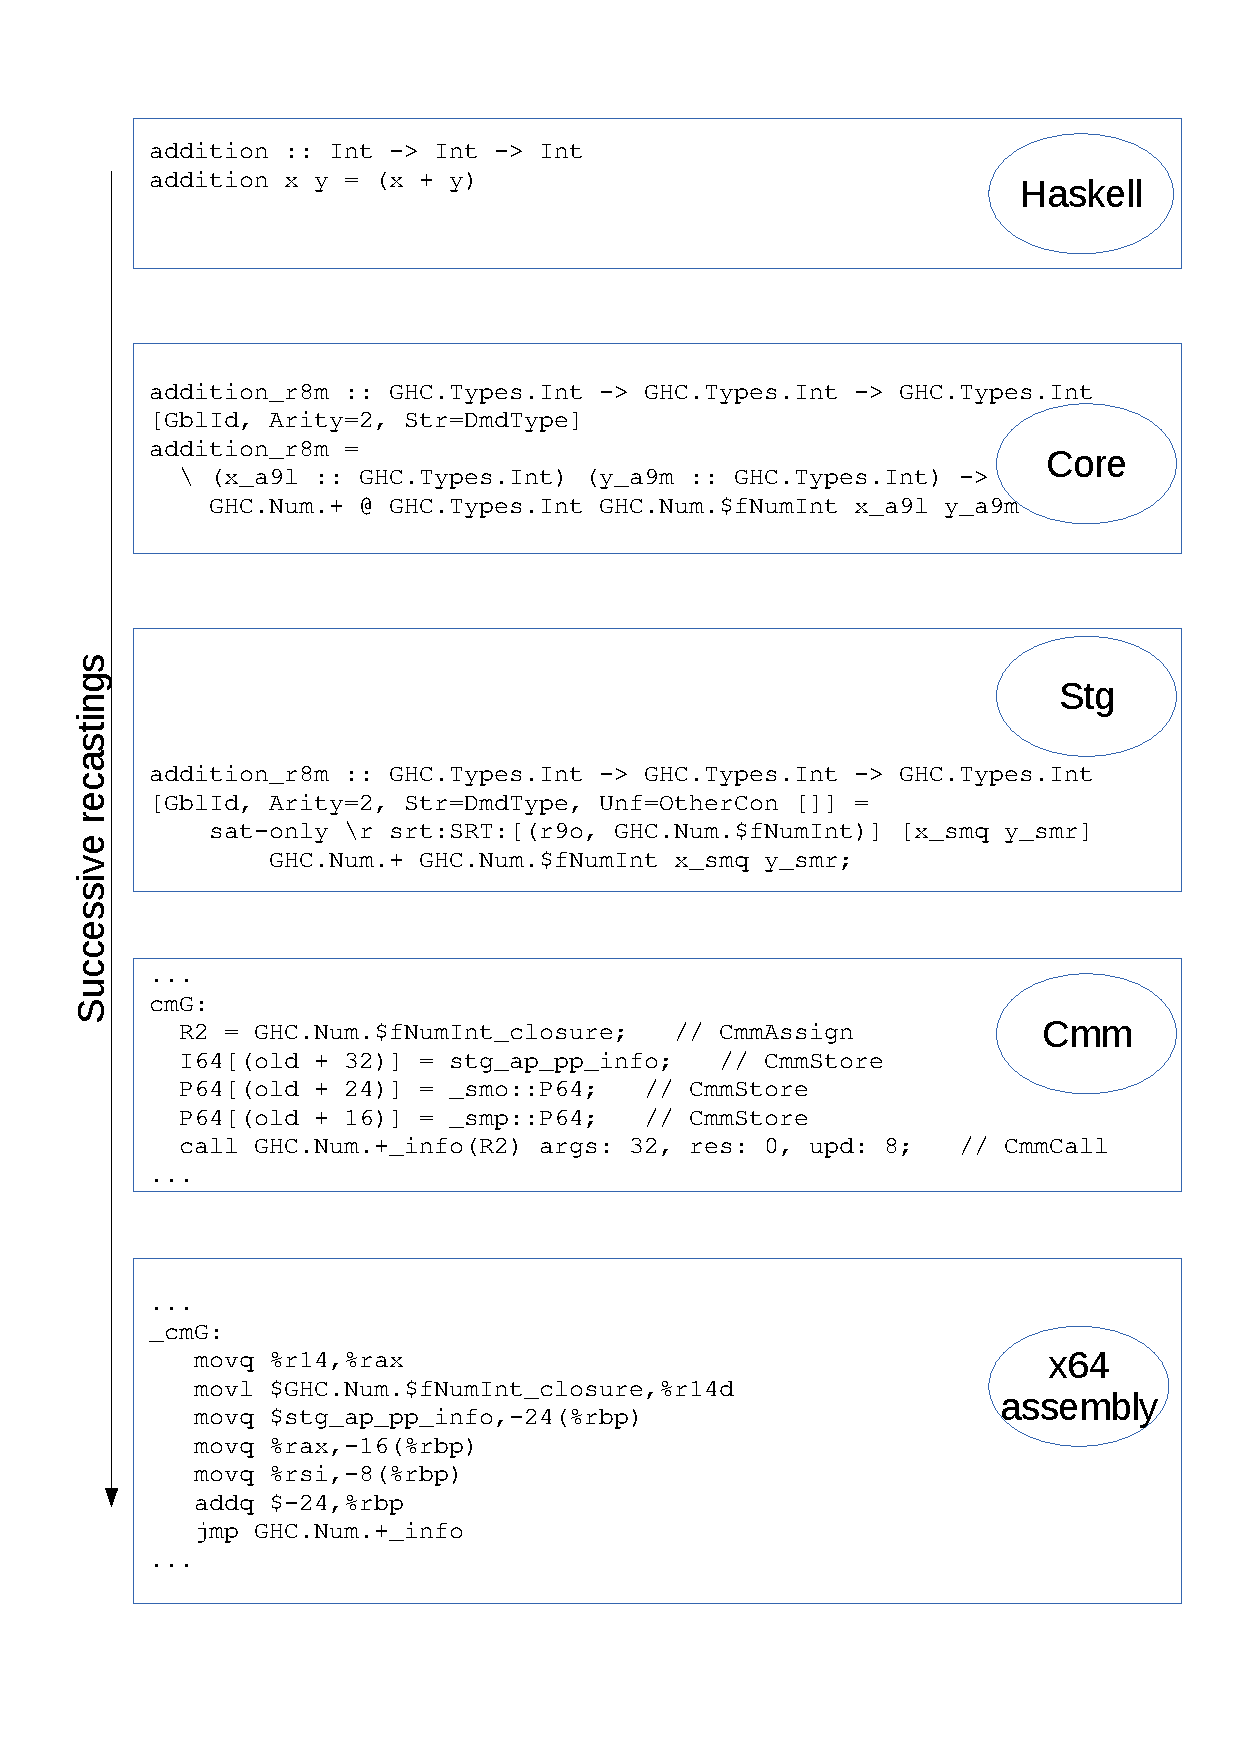
\includegraphics[width=5.5in]{fig/recastings}
  \caption{The IRs in GHC for a simple function. The assembly is also
  included even tough it is not an intermediate representation (it is
  the final representation)}\label{fig:recastings}
\end{mdframed}
\end{figure}

\subsubsection{The STG IR}

There is nothing that says that Haskell must be implemented using some
sort of stack. In section \ref{sec:stack_in_GHC} we saw that GHC, one
popular Haskell compiler, chooses to implement the language using a
stack called the execution stack. The STG intermediate representation
in GHC is interesting to us since it is a representation of code where
it is specified how it will interact with the execution stack. The STG
code in \ref{fig:recastings} does not have a clean syntax, instead we
use the syntax from the Ministg project \cite{haskellwiki_ministg}.
Figure \ref{fig:haskell_vs_ministg} shows Haskell code and the
corresponding Ministg code. In the Haskell world, \texttt{doubleAddition} and
\texttt{globalThunk} are both just values, in theory we do not really
know if multiple uses of \texttt{globalThunk} will be memoized. Such
implementation details are not relevant in the Haskell world.
Looking at the STG however, we can be sure if the value
\texttt{globalThunk} will be memoized or not. By examining the STG code
in figure \ref{fig:ministg} we can make the following observations.

\begin{figure}
\begin{mdframed}
        \begin{subfigure}[t]{1\textwidth}
          \begin{minted}{haskell}
doubleAddition :: Int -> Int -> Int
doubleAddition x y = tot + tot
  where tot = x + y

globalThunk :: Int
globalThunk = doubleAddition 2 3
          \end{minted}
          \caption{Haskell code}
        \end{subfigure}
        \vskip2em
        \begin{subfigure}[t]{1\textwidth}
          \begin{minted}{haskell}
doubleAddition = FUN(x y ->
    let { tot = THUNK(plusInt x y);
        }
    in plusInt tot tot);

globalThunk = THUNK(doubleAddition two three);

-- And some imported functions

two = CON(I 2);
three = CON(I 3);

plusInt = FUN(x y -> ... ); -- Definition omitted
          \end{minted}
          \caption{STG code with the Ministg syntax}
          \label{fig:ministg}
        \end{subfigure}
  \caption{Haskell code and STG code}
  \label{fig:haskell_vs_ministg}
\end{mdframed}
\end{figure}

\begin{itemize}
  \item
    The implementation of \texttt{doubleAddition} is a function that
    takes two arguments, as expected\footnote{It could in theory be a
      function taking one argument returning another function of one
      argument.}.
  \item
    The value of \texttt{tot} is put into one thunk. Another possible
    implementation would have been to inline it to \texttt{x + y + x +
      y}. This would be worse in fact, because it would then actually
    require to create \emph{two} thunks instead. One for \texttt{(x +
      y)} and one for \texttt{((x + y) + x)}.
  \item
    The value \texttt{globalThunk} will be a thunk. When a thunk is
    defined at the top level, it can become a \emph{global thunk}.
    A global thunk will only be evaluated at most once during the
    execution of a Haskell program. Some Haskell programmers are more
    familiar with the term CAF or constant applicative form. In this
    thesis we call them global thunks.
  \item
    We are also reminded that literals like \texttt{2} and \texttt{3}

\end{itemize}

The experienced Haskell programmer will know all of this by heart
by looking at the Haskell code (in this case, the programmer was so
confident that he named the value \texttt{globalThunk} with such a
suggestive name!). However, the only way to be certain is
to look at the intermediate code that GHC emits.


\subsection{Generating debug data}

There is one common complex problem that must be solved to enable debugging
tools: The programmer thinks of the program as its source code and the
semantics of the language. However, the processor only runs machine code.
Unfortunately, there is no way to associate the machine code to the
source code that it originated from. This is a problem for all applications of
debugging, not limited to stack traces \cite{eager2012introduction}. As a consequence, any
compiler that wants to support debugging has to do the truly overwhelming task of threading along
information about the original source code that got compiled into each
intermediate step, this information must also be retained and transformed
accordingly during all the optimization steps. Figure
\ref{fig:recastings_ticks} shows
debug information that have been retained through all the transformations in
the GHC pipeline when compiling a simple function.

\begin{figure}
\begin{mdframed}
  \centering
  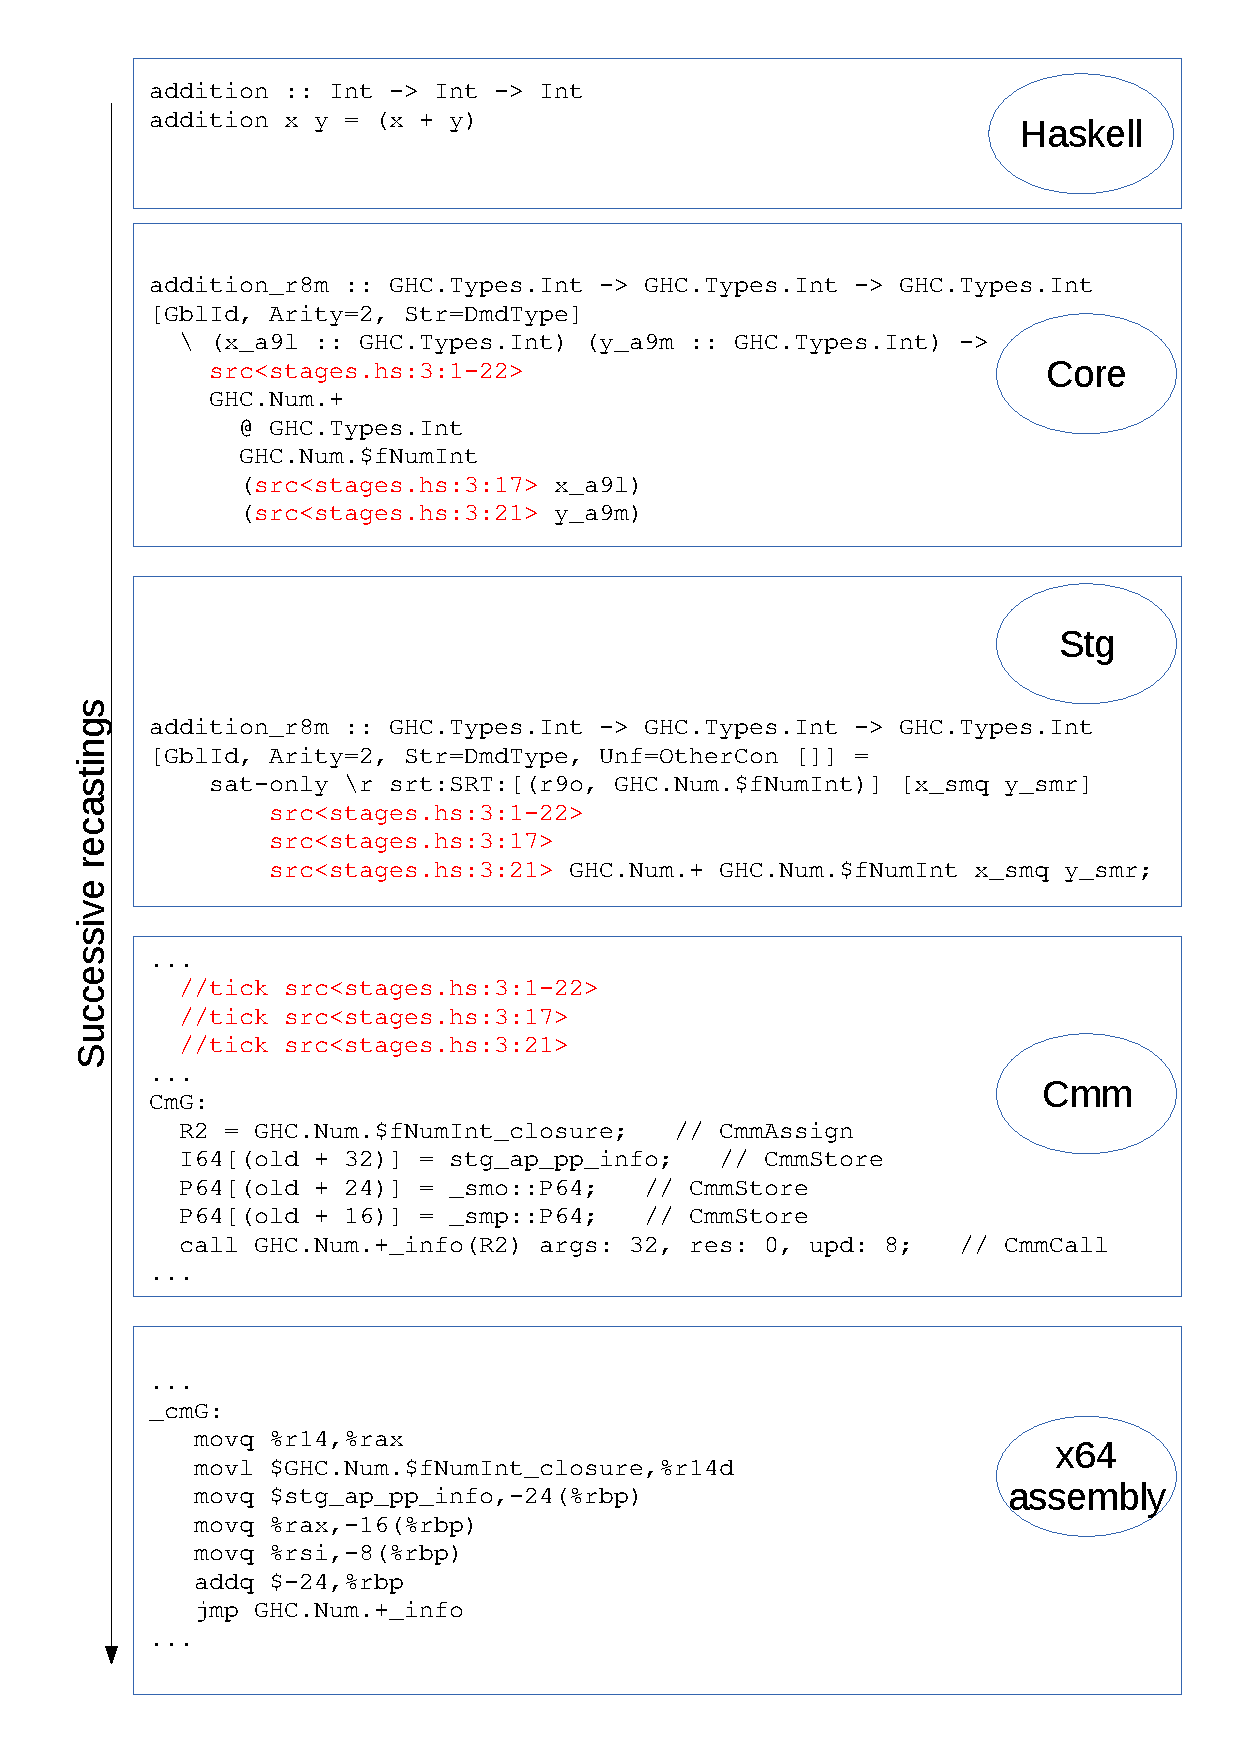
\includegraphics[width=5.4in]{fig/recastings_ticks}
  \caption{The same figure as \ref{fig:recastings}, only that here each
  IR has debug data attached to it. The debug data tells us what Haskell
  source code the IR code is compiled from. For clarity the debug data
  annotations have a red font.}
  \label{fig:recastings_ticks}
\end{mdframed}
\end{figure}

One important observation is that
any implementation can only be a best effort implementation.
Consider figure \ref{fig:same_functions} which contains two Haskell functions
with \emph{exactly} the same implementation. A clever compiler will
be able to realize that the two function bodies are identical,
it would then be safe for the compiler to remove one of the functions
and just change the call sites of the removed function to use the other function.
But this has a drawback because a stack trace
involving the removed function can not exist. Figure
\ref{fig:optimization} highlights this problem, Haskell can't
report which function caused the crash, since that
function is optimized away. In conclusion, an implementation of stack traces that have no
effect on performance can only be a best effort attempt.

\begin{figure}
\begin{mdframed}
  \begin{minted}{haskell}
kilometerToMeter = (*1000)
kilogramToGram = (*1000)
  \end{minted}
  \caption{Two functions with identical implementations. }
  \label{fig:same_functions}
\end{mdframed}
\end{figure}

\begin{figure}
\begin{mdframed}
        \begin{subfigure}[t]{0.5\textwidth}
            \begin{minted}{haskell}
reciprocal_1 :: Int -> Int
reciprocal_1 x = 1 `div` x

reciprocal_2 :: Int -> Int
reciprocal_2 = (1 `div`)

main = do
  print (reciprocal_1 5)
  print (reciprocal_2 0) -- crash!
            \end{minted}
            \caption{Original program.}
        \end{subfigure}
        ~ %add desired spacing between images, e. g. ~, \quad, \qquad etc.
          %(or a blank line to force the subfigure onto a new line)
        \begin{subfigure}[t]{0.5\textwidth}
          \begin{minted}{haskell}
reciprocal_1 :: Int -> Int
reciprocal_1 x = 1 `div` x

main = do
  print (reciprocal_1 5)
  print (reciprocal_1 0) -- crash!
          \end{minted}
          \caption{After optimizations.}
        \end{subfigure}
        \caption{An example showing why optimizations can give
        inaccurate stack traces.}\label{fig:optimization}
\end{mdframed}
\end{figure}

Finally, the information about the source-level functions that the compiler
have held tight throughout the IRs must get packaged into the binary. This
concern arises naturally in the final IR stage (Cmm in the case of GHC).  How does the compiler emit the
debug information? How is it stored in a way so it doesn't get in the way of the
actual code?  A debugging format answers these questions. One such debugging
format is DWARF.

\section{DWARF}

In 1988, DWARF was created hoping to solve a quite general problem. DWARF is
a language agnostic debugging format that is still producing updated revisions.
DWARF 5 is planned to be released in 2014. \cite{eager2012introduction} The DWARF data that is
stored in the binary can be understood by a debugger like \texttt{gdb}. For example,
it could help gdb explain how some data should be displayed, for instance if a
particular byte is a 8-bit number or a character.

Looking at figure \ref{fig:recastings_ticks} again, we see that
the first phase (the original Haskell source code) nor the last
phase (the output assembly) has any debug information attached to
it. This does make sense because the programmer should not need to
annotate their source code to get stack traces, neither should the
performance of the program degrade by changing the output assembly.
But then where is the final debug data emitted? It must be included
with the binary of course. The binary is divided into \emph{sections}
\cite{oracle_object_file_format}, some of these sections are DWARF
sections. The command line tool \texttt{dwarfdump} can inspect the
DWARF data in object files. Figure \ref{fig:dwarfdump} show some of the
DWARF data that GHC included in the object file it created. The figure
shows only some of the relevant debug information, for example, the line
numbers are not stored anywhere in the contents of the figure.

\begin{figure}
\begin{mdframed}
  \begin{minted}{text}
< 1><0x0000008d>    DW_TAG_subprogram
                      DW_AT_name                  "addition"
                      DW_AT_MIPS_linkage_name     "r8m_info"
                      DW_AT_external              no
                      DW_AT_low_pc                0x00000020
                      DW_AT_high_pc               0x00000054
                      DW_AT_frame_base            DW_OP_call_frame_cfa
< 2><0x000000b3>      DW_TAG_lexical_block
                        DW_AT_name                  "cmG_entry"
                        DW_AT_low_pc                0x00000029
                        DW_AT_high_pc               0x0000004b
< 2><0x000000cf>      DW_TAG_lexical_block
                        DW_AT_name                  "cmF_entry"
                        DW_AT_low_pc                0x0000004b
                        DW_AT_high_pc               0x00000054
  \end{minted}
  \caption{The DWARF data generated from the debug annotations in figure
    \ref{fig:recastings_ticks}.}
  \label{fig:dwarfdump}
\end{mdframed}
\end{figure}

% TODO: Write about the instruction pointer to source code mapping?

As will be revealed in
section \ref{sec:recent_work}, this thesis work was made possible thanks
to that DWARF got integrated in GHC.

\chapter{Related work} \label{chp:related_work}

To programmers outside of the Haskell community, it could sound
surprising that a mature language like Haskell doesn't support stack
traces. This might raise the following questions:

\begin{itemize}
  \itemsep1pt\parskip0pt\parsep0pt
  \item
    Since stack traces are difficult, what other means of debugging are
    there?
  \item
    Are stack traces in Haskell really necessary?
  \item
    Is there at least any inefficient way to get stack traces?
  \item
    How close is the Haskell community in solving stack traces?
\end{itemize}

The overall structure of this chapter is that we answer the questions
by looking at related work. Most of the
related work is recent, usually less than 5 years from the time of
publishing of this work. The first question is answered in section
\ref{sec:debugging_haskell}. Section \ref{sec:avoiding_crashing}
shows that Haskell is a language producing robust programs, which
alleviates the need for stack traces.
The third question is answered in section
\ref{sec:overhead_full} which shows many working implementations of
stack traces, all of which have significant overhead. The last question
is answered in section \ref{sec:recent_work}.

\section{Debugging Haskell} \label{sec:debugging_haskell}

Examining stack traces falls in the category of debugging. Programmers
examine stack traces printed from a handled exception or a
crash. The amount of time the program runs before it crashes can be
anywhere between a few nanoseconds to many years. Stack traces are most
valuable for programs that crash unexpectedly after a long time of
stable execution, because it might be hard to reproduce the error in
order to diagnose it. Ideally, the stack trace aids the programmer in
writing a minimal reproducible test case that exercises the original
bug. Once programmers have an easy to reproduce bug, they look for
tools that help them better understand why the bug is happening. In this
subsection we'll look at existing tools for GHC that let programmers
step through the program's execution and even print variables. Neither of
which the stack trace implementation in this paper can provide.

\subsection{GCHi Debugger}

GHC comes with its own interactive \emph{read evaluate print loop} (REPL)
which has an built-in debugger. It's rich in features, supporting break
points, single-stepping, breaking on crashes, a "tracing mode" and even
variable inspection. The implementation works only with interpreted
code \cite{marlow2007lightweight, ghci_debugger}. So there will be significant overhead both
from the fact that the code is interpreted and that the debugger is
running.


\subsection{ghc-vis}

Debuggers are a view into the otherwise opaque executing program. The
GHCi debugger interface is text based, the programmer enters a command
to the debugger and it responds in text.  ghc-vis on the other hand is a
graphical debugger.  It allows users to visualize variables and interact
with them with the mouse pointer. For example, when clicking on an yet
unevaluated expression (remember, Haskell is a lazy language) it will
evaluate the expression.  Making it great for stepping through your
program without losing the big picture.  ghc-vis is hooking itself into
the program by running a thread inside of ghci. So it will only work
with ghci.  \cite{thesisFelsingBA}

\section{Avoiding Crashing} \label{sec:avoiding_crashing}

If a program never crashes,
it will not matter if our language prints stack traces or not. Never-crashing programs is a research area, sometimes called formal
verification. There are many approaches to formal verification. One
can statically analyze C-programs \cite{ckl2004},
use finite automata
or formal grammars \cite{dantam2013motion, rouhani2013software},
use type system tricks \cite{cheney2003first}
or use total functional programming \cite{Turner:jucs_10_7:total_functional_programming}.
In the end tough, none of the these methods are perfect, otherwise we
would not need stack traces.

There are also statical analysis tools for Haskell. HALO is a tool
where the programmers writes contracts about their own programs and
then lets HALO prove them \cite{vytiniotis2013halo}. HALO seems to
be inspired from \cite{xu2009static} which in turn is inspired by
\cite{xu2006extended}. Another tool is HipSpec which does automatic
proof finding instead of having the programmer spell out the properties
to validate \cite{claessen2013automating}. Yet another tool that's
mentioned on Haskellwiki is Catch where its described to "detect common
sources of runtime errors" \cite{haskellwiki_static_analysis_tools}.

\subsection{Catch}

Catch is a static analyzer for Haskell. It can detect if a pattern-matching is
sufficiently covering, even if the cases aren't collectively exhaustive. Figure
\ref{fig:catch_example} shows a function where the pattern match isn't exhaustive but
sufficiently so.
Catch can prove that such a pattern
matching is safe by doing flow analysis and ruling out impossible
patterns for the scrutiny (the expression that we \texttt{case} on).
This eliminates the need for the human programmer to manually check what can be
automatically proven. \cite{mitchell:catch_2008_9_25}

\begin{figure}
\begin{mdframed}
      \begin{minted}{haskell}
safeFunction = nonExhaustivePatterns False
  where
    nonExhaustivePatterns False = 42
      -- NOTE: No pattern for True
      \end{minted}
      \caption{A safe function even though the non-exhaustive matching. A
        totality checker like Catch can ensure that it's safe.}
      \label{fig:catch_example}
\end{mdframed}
\end{figure}

\section{Inefficient stack traces} \label{sec:overhead_full}

There are already many successful stack trace implementations in
Haskell. Unfortunately, they all have a significant overhead.
In this section we will look at previous work about stack traces for
Haskell. There are two common sources of overhead in existing implementations:

\begin{itemize}
\itemsep1pt\parskip0pt\parsep0pt
\item
  By building an explicit call stack (Subsection \ref{sec:explicit_call_stack})
\item
  By depending on expensive runtime settings (Subsection \ref{sec:stack_traces_with_profiling})
\end{itemize}

\subsection{Explicit call stack} \label{sec:explicit_call_stack}

Stack traces can be achieved by doing some methodological source level
transformations. Figure \ref{fig:transformation} shows a program transformed
into one producing stack traces on calls to \texttt{error}. This transformation is essentially:

\begin{itemize}
\itemsep1pt\parskip0pt\parsep0pt
\item
  Changing all top level functions to take one additional string
  argument. Except for the program entry-point \texttt{main}.
\item
  Transform all equations to define the new call stack \texttt{stack'} and
  pass it as the first argument to all calls of top level functions.
\item
  Transform all calls to \texttt{error} to also print out the call stack.
\end{itemize}

This transformation is similar to \cite{source_transformation} and a
complete source-to-source implementation called \emph{hat} exists already
\cite{hat_website}. But explicit call stack implementations don't need
to work on a source level.

\begin{figure}
\begin{mdframed}
        \begin{subfigure}[t]{0.4\textwidth}
            \begin{minted}{haskell}
main = print (f 100)

f :: Int -> Int
f x = g (5*x)

g :: Int -> Int
g 7 = error "Bang"
g x = 100 * x
            \end{minted}
            \caption{Original program}
        \end{subfigure}
        ~ %add desired spacing between images, e. g. ~, \quad, \qquad etc.
          %(or a blank line to force the subfigure onto a new line)
        \begin{subfigure}[t]{0.6\textwidth}
          \begin{minted}{haskell}
main = print (f stack' 100)
  where
    stack' = "main \n"

f :: String -> Int -> Int
f stack x = g stack' (5*x)
  where
    stack' = "f (case 1)\n" ++ stack

g :: String -> Int -> Int
g stack 7 = error ("Bang" ++ stack')
  where
    stack' = "g (case 1)\n" ++ stack
g stack x = 100 * x
  where
    stack' = "g (case 2)\n" ++ stack
          \end{minted}
          \caption{Transformed program}
        \end{subfigure}
        \caption{An example of how a Haskell program can be transformed to one
          that will print stack traces on errors. The syntax `\texttt{str1 ++
            str2}' is string concatenation.
        }\label{fig:transformation}
\end{mdframed}
\end{figure}

\subsubsection{StackTrace}

Allwood et al implemented a Intermediate Representation (IR) transformation
pass called \emph{StackTrace}. It's operating on the GHC Core IR. Since
Core is like a small subset of Haskell, its implementation will do
something similar to what figure \ref{fig:transformation} illustrates.

Among its complications are the
handling of higher order functions, linking with code that doesn't have stack
traces and an efficient non-naive implementation of the
passed along stack \cite{FindingTheNeedle2009}.
Functional programming in particular relies on efficient tail call
optimizations, which
requires the passed around call stack to efficiently handle this.

% TODO, Detta (ContMarks) passar inte in alltså, iom allt annat har med just
% Haskell att göra plus att det ska vara om overhead-full stack traces.
% detta borde ju bli overhead-full men svårt att bara påstå det.
% \subsubsection{Continuation Marks}

% The other dimensionality of complications is the implementation
% complexity.  There are other debugging features besides stack traces a
% compiler would like to support, and the more features the bigger blowup
% in the complexity of the compiler itself.  Clements disseratation shows
% a framework called \emph{continuation marks} which allows for a generic
% way to create addons to the language \cite{clements_dissertation2005}.
% In his disseratation, he uses continuation marks as a common ground of
% implementation for stack traces, code stepping in debugging and aspect
% oriented programming.  Since GHC does not have continuation marks
% implemented, it's not a possible starting point for implementing stack
% traces.

\subsection{Stack traces with profiling} \label{sec:stack_traces_with_profiling}

A mature and stable implementation of stack traces for
Haskell is present in GHC since GHC 7.4.1 which was released in February
2012. No paper has been produced from this effort. But a talk were
given at Haskell Implementors Workshop in September 2012 \cite{HIW2012Programme}.
The implementation is only working in conjunction with the profiling
mode of GHC. In Profiling mode the execution of programs can expect to
be twice as slow as their plain counterparts. The cost centre stack traces
have its own set of problems and is only an approximation of what Haskell
really is executing.

\section{Recent work} \label{sec:recent_work}

Around the time when this thesis started, Peter Wortmann, a
PhD candidate at University of Leeds showed a proof of concept
stack trace in Haskell that was based on the execution stack
\cite{stack_traces_ticket}. Peter had been working on non intrusive
profiling for GHC. To accomplish this, he had developed a theory of
causality of computations in Haskell and his work extended even to
optimized code \cite{DBLP:conf/haskell/WortmannD13}. To do profiling
he needed to map instruction pointers to the corresponding source
code. He added source code annotations that propagated
through the pipeline of IRs and optimizations and finally emitted DWARF
debugging data. Figure \ref{fig:core_and_ticks} shows how a code
annotation has been placed in the Core IR. With his patches, GHC now
emits DWARF, making a stack trace implementation to be low hanging
fruit, enabling the quite sizeable problem of stack traces to be worked
on during the limited scope of a master's thesis.

\begin{figure}
\begin{mdframed}
        \begin{subfigure}[t]{0.4\textwidth}
            \begin{minted}{text}
$wfibonacci =
  \ (ww_spO :: Int#) ->
    case ww_spO of ds_Xph {
      __DEFAULT -> ...
            \end{minted}
            \caption{Without ticks, the default option}
        \end{subfigure}
        ~ %add desired spacing between images, e. g. ~, \quad, \qquad etc.
          %(or a blank line to force the subfigure onto a new line)
        \begin{subfigure}[t]{0.6\textwidth}
          \begin{minted}{text}
$wfibonacci =
  \ (ww_spO :: Int#) ->
    src<0:Fibonnaci.hs:(4,1)-(6,51)>
    case ww_spO of ds_Xph {
      __DEFAULT -> ...
          \end{minted}
          \caption{With ticks by passing the flags \texttt{-g -dppr-ticks}}
        \end{subfigure}
        \caption{The same excerpt of the Core generated from the program
in figure \ref{fig:simple_program}. Only the version on the right have
debug data included }\label{fig:core_and_ticks}
\end{mdframed}
\end{figure}

But the original stack traces produced from Peter's simple demo
isn't satisfactory. The output from running the program in figure
\ref{fig:sample_program} could look like \ref{fig:trace_goal1}. This
work is partially motivated by trying to make the stack look more like
\ref{fig:trace_goal2}.

\begin{figure}
\begin{mdframed}
  \begin{minted}{haskell}
main :: IO ()
main = do print 1
          a
          print 2

a, b, c :: IO ()
a = do print 10
       b
       print 20

b = do print 100
       c
       print 200

c = do print 1000
       print (crashSelf 2)
       print 2000

crashSelf :: Int -> Int
crashSelf 0 = 1 `div` 0
crashSelf x = crashSelf (x - 1)
  \end{minted}
  \caption{A sample Haskell program that will crash when run}
  \label{fig:sample_program}
\end{mdframed}
\end{figure}




\begin{figure}
\begin{mdframed}
  \begin{subfigure}[t]{0.5\textwidth}
    {\small
    \begin{minted}{text}
 0: stg_bh_upd_frame_ret
 1: stg_bh_upd_frame_ret
 2: stg_bh_upd_frame_ret
 3: showSignedInt
 4: stg_upd_frame_ret
 5: writeBlocks
 6: stg_ap_v_ret
 7: bindIO
 8: bindIO
 9: bindIO
10: bindIO
11: stg_catch_frame_ret
    \end{minted}
  }%
    \caption{A stack trace, clearly based on the execution stack. Since the
      execution stack is bound to GHC's specific implementation of Haskell,
      it'll be difficult for programmers to interpret.}
    \label{fig:trace_goal1}
  \end{subfigure}
        ~ %add desired spacing between images, e. g. ~, \quad, \qquad etc.
          %(or a blank line to force the subfigure onto a new line)
        \begin{subfigure}[t]{0.5\textwidth}
    {\small
          \begin{minted}{text}
 0: crashSelf
 1: crashSelf
 2: print
 3: c
 4: b
 5: a
 6: main
          \end{minted}
  }%
          \caption{An ideal, fictive, stack trace, without
          implementation details of the execution stack. It's rather a
          semantic stack.}
          \label{fig:trace_goal2}
        \end{subfigure}
        \caption{Two stack traces
        }\label{fig:traces}
\end{mdframed}
\end{figure}

 % Not for the planning report
